\documentclass[a4paper,10pt]{article}
\usepackage{amsmath}
\usepackage{amsfonts}
\usepackage{graphicx}
\usepackage{color}
\usepackage{float}

\title{CS532100 Numerical Optimization Homework 2}
\author{109062710 Bijon Setyawan Raya}
\date{Due Dec 10}
\begin{document}
\maketitle
\begin{enumerate}
    \item Consider the linear least square problem:
    \[ 
        \min_{\vec{x}\in \mathbb{R}^2}||A\vec{x} - \vec{b}||^2
    \]
    where
    \[
        A = \left[ \begin{array}{cc}4 & 8 \\ 2 & 4 \\ 1 & 2 \end{array} \right], 
        \vec{b} = \left(\begin{array}{c} 21/4 \\ 0 \\ 0 \end{array} \right)
    \]

\begin{enumerate}
	\item (10\%) Write its normal equation.
    {\color{blue} 
        \begin{align}
            A^T A \vec{x} &= A^T \vec{b} \\
            \begin{bmatrix}4 & 2 & 1 \\ 8 & 4 & 2\end{bmatrix} \begin{bmatrix}4 & 8 \\ 2 & 4 \\ 1 & 2\end{bmatrix} \begin{bmatrix} x_1 \\ x_2 \end{bmatrix} &= \begin{bmatrix}4 & 2 & 1 \\ 8 & 4 & 2\end{bmatrix} \begin{bmatrix}21/4 \\ 0 \\ 0\end{bmatrix} \\
            \begin{bmatrix} 1 & 2 \\ 2 & 4 \end{bmatrix} \begin{bmatrix} x_1 \\ x_2 \end{bmatrix} &= \begin{bmatrix} 1 \\ 2 \end{bmatrix} \\
            x_1 + 2x_2 = 1
        \end{align}

        Then, we can express $x_1$ and $x_2$ as
        \begin{align}
            \vec{x} = \begin{bmatrix} 1-2t \\ t \end{bmatrix}
        \end{align}
    }

    \item (10\%) Express $\vec{b} = \vec{b}_1 + \vec{b}_2$ such that $\vec{b}_1$ is in the subspace spanned by $A$'s column vectors, and $\vec{b}_2$ is orthogonal to $A$'s column vectors.
    {\color{blue} 
        From matrix A, we know that its basis is its first column which is $\begin{bmatrix}4 & 2 & 1\end{bmatrix}^T$. 
        From its basis column, we can express $\vec{b}$ in $\vec{b}_1 + \vec{b}_2$.

        Let, 
        \begin{align}
            \vec{b}_1 = \begin{bmatrix}4s \\ 2s \\ s\end{bmatrix}, \vec{b}_2 = \begin{bmatrix}t_1 \\ t_2 \\ t_3\end{bmatrix}
        \end{align}

        Then we can express $\vec{b}$ such as 
        \begin{align}
            \vec{b} &= \vec{b}_1 + \vec{b}_2 \\
            \begin{bmatrix}21/4 \\ 0 \\ 0\end{bmatrix} &= \begin{bmatrix}4s + t_1 \\ 2s + t_2 \\ s + t_3\end{bmatrix}
        \end{align}

        Since $\vec{b}_1$ is a column space of A, and $\vec{b}_2$ is orthogonal to $\vec{b}_1$, then
        \begin{align}
            \begin{bmatrix}4s \\ 2s \\ s\end{bmatrix} \begin{bmatrix}t_1 & t_2 & t_3\end{bmatrix} &= 0 \\ 
            4s \cdot t_1 + 2s \cdot t_2 + s \cdot t_3 &= 0
        \end{align}

        We can add $4s \cdot t_1 + 2s \cdot t_2 + s \cdot t_3 = 0$ at the last index of our matrix equality. Then
        \[
        \begin{bmatrix} 4s + t_1 \\ 2s + t_2 \\ s + t_3 \\ 4s \cdot t_1 + 2s \cdot t_2 + s \cdot t_3\end{bmatrix} = \begin{bmatrix} 21/4 \\ 0 \\ 0 \\ 0 \end{bmatrix}
        \]

        Solving the equality above, we then have $s = 1$, $t_1 = 5/4$, $t_2 = -2$, and $t_3 = -1$. Thus, 
        \begin{align}
            \vec{b}_1 = \begin{bmatrix}4s \\ 2s \\ s\end{bmatrix}, \vec{b}_2 = \begin{bmatrix}5/4 \\ -2 \\ -1\end{bmatrix} \\ 
            \begin{bmatrix}21/4 \\ 0 \\ 0\end{bmatrix} = \begin{bmatrix}4 \\ 2 \\ 1\end{bmatrix} + \begin{bmatrix}5/4 \\ -2 \\ -1\end{bmatrix}
        \end{align}
    }

    \item (10\%) Show that $\vec{z}\in \mathbb{R}^2$ is a least square solution for $A\vec{x}=\vec{b}$ if and only if $\vec{z}$ is part of a solution to the larger linear system:
    \[
        \left[ \begin{array}{cc}0 & A^T \\ A & I\end{array} \right] \left[\begin{array}{cc} \vec{z} \\ \vec{y} \end{array}\right] = \left[\begin{array}{cc} 0 \\ \vec{b}\end{array}\right]
    \]
    {\color{blue}
        We are going to show that $\vec{z}\in \mathbb{R}^2$ is a least square solution for $A\vec{x}=\vec{b}$ $\iff$ $\vec{z}$ is part of a solution to the larger linear system
        \begin{enumerate}
        \item
            First, we are going to show that if $\vec{z}\in \mathbb{R}^2$ is a least square solution for $A\vec{x}=\vec{b}$ then $\vec{z}$ is part of a solution to the larger linear system.
            
            \begin{align}
                A\vec{x} &= \vec{b} \\
                A^T A \vec{x} &= A^T \vec{b} \\
                \begin{bmatrix}4 & 2 & 1 \\ 8 & 4 & 2\end{bmatrix} \begin{bmatrix}4 & 8 \\ 2 & 4 \\ 1 & 2\end{bmatrix} \begin{bmatrix} x_1 \\ x_2 \end{bmatrix} &= \begin{bmatrix}4 & 2 & 1 \\ 8 & 4 & 2\end{bmatrix} \begin{bmatrix}21/4 \\ 0 \\ 0\end{bmatrix} \\
                \begin{bmatrix} 1 & 2 \\ 2 & 4 \end{bmatrix} \begin{bmatrix} x_1 \\ x_2 \end{bmatrix} &= \begin{bmatrix} 1 \\ 2 \end{bmatrix} \\
                x_1 + 2 x_2 = 1
            \end{align}
    
            Then, we can express $x_1$ and $x_2$ as
            \begin{align}
                \vec{x} = \begin{bmatrix} 1-2t \\ t \end{bmatrix}
            \end{align}

            Plugging $\vec{x}$ into $\vec{z}$ in the larger linear system, we then have
            \begin{align}
                \begin{bmatrix} 0 & A^T \\ A & I \end{bmatrix} \begin{bmatrix} \vec{z} \\ \vec{y} \end{bmatrix} &= \begin{bmatrix} 0 \\ \vec{b} \end{bmatrix} \\
                \begin{bmatrix} 0 & 0 & 4 & 2 & 1 \\ 0 & 0 & 8 & 4 & 2 \\ 4 & 8 & 1 & 0 & 0 \\ 2 & 4 & 0 & 1 & 0 \\ 1 & 2 & 0 & 0 & 1 \end{bmatrix} \begin{bmatrix} 1-2t \\ t \\ \vec{y}_1 \\ \vec{y}_2 \\ \vec{y}_3 \end{bmatrix} &= \begin{bmatrix} 0 \\ 0 \\ 21/4 \\ 0 \\ 0 \end{bmatrix}
            \end{align}

            Solving $\vec{y}$, we have
            \begin{align}
                \vec{y} = \begin{bmatrix}5/4 \\ -2 \\ -1\end{bmatrix}
            \end{align}

            From $\vec{y}$, we can tell that $\vec{z}\in \mathbb{R}^2$ is a least square solution for $A\vec{x}=\vec{b}$.

            Thus, the premise, if $\vec{z}\in \mathbb{R}^2$ is a least square solution for $A\vec{x}=\vec{b}$ then $\vec{z}$ is part of a solution to the larger linear system, holds.
            

        \item
            Second, we are going to show that if $\vec{z}$ is a part of the solution to the larger linear system then $\vec{z}\in \mathbb{R}^2$ is a least square solution for $A\vec{x}=\vec{b}$.
            
            The larger linear system can be expressed as
            \begin{align}
                \begin{bmatrix} 0 & A^T \\ A & I \end{bmatrix} \begin{bmatrix} \vec{z} \\ \vec{y} \end{bmatrix} &= \begin{bmatrix} 0 \\ \vec{b} \end{bmatrix} \\
                \begin{bmatrix} 0 & 0 & 4 & 2 & 1 \\ 0 & 0 & 8 & 4 & 2 \\ 4 & 8 & 1 & 0 & 0 \\ 2 & 4 & 0 & 1 & 0 \\ 1 & 2 & 0 & 0 & 1 \end{bmatrix} \begin{bmatrix} \vec{z}_1 \\ \vec{z}_2 \\ \vec{y}_1 \\ \vec{y}_2 \\ \vec{y}_3 \end{bmatrix} &= \begin{bmatrix} 0 \\ 0 \\ 21/4 \\ 0 \\ 0 \end{bmatrix}
            \end{align}
            
            Solving $y_1$, $y_2$, and $y_3$, we express them as
            \begin{align}
                \vec{y} = \begin{bmatrix} 5/4 \\ -2 \\ -1 \end{bmatrix}
            \end{align}

            After acquiring $\vec{y}$, we can acquire $\vec{z}$ with the third, the fourth, and the fifth row in the matrix. Thus,
            \begin{align}
                4\vec{z}_1 + 8\vec{z}_2 + \vec{y}_1 &= \frac{21}{4} \\ 
                2\vec{z}_1 + 4\vec{z}_2 + \vec{y}+2 &= 0 \\
                \vec{z}_1 + 2\vec{z}_2 + \vec{y}_3 &= 0
            \end{align}

            Solving the equalities above, we have 
            \begin{align}
                \vec{z}_1 + 2\vec{z}_2 = 1
            \end{align}

            We can express the equality above in matrix as,
            \begin{align}
                \vec{z} = \begin{bmatrix} 1 - 2t \\ t \end{bmatrix}
            \end{align}
            Clearly, $\vec{z}$ is a part of the solution to the larger linear system.
            
            Thus, the premise, if $\vec{z}$ is a part of the solution to the larger linear system then $\vec{z}\in \mathbb{R}^2$ is a least square solution for $A\vec{x}=\vec{b}$, holds.
        \end{enumerate}

        By showing the premises above, we can conclude that the statement, $\vec{z}\in \mathbb{R}^2$ is a least square solution for $A\vec{x}=\vec{b}$ if and only if $\vec{z}$ is part of a solution to the larger linear system, holds.
    }

\end{enumerate}
    \item In Note05 (Page 16), memoryless BFGS iteration matrix $H_{k+1}$ can be derived from considering the Hestenes–Stiefel form of the nonlinear conjugate gradient method. Recalling that $\vec{s}_k = \alpha_k \vec{p}_k$, we have that the search direction for this method
is given by
\begin{align}
    \vec{p}_{k+1} &= -\nabla f_{k+1} + \frac{\nabla f_{k+1}^T\vec{y}_k}{\vec{y}^T\vec{p}_k}\vec{p}_k \\
    &= -\nabla f_{k+1} + \frac{\nabla f_{k+1}^T\vec{y}_k}{\vec{y}^T\vec{s}_k}\vec{s}_k \\ 
    &= -( I - \frac{\vec{s}_k\vec{y}_k^T}{\vec{y}^T\vec{s}_k})\nabla f_{k+1} \\ 
    &= - \hat{H}_{k+1} \nabla f_{k+1}
\end{align}
However, the matrix $\hat{H}_{k+1}$ is neither symmetric nor positive definite.
\begin{enumerate}
    \item (10\%) Please show that the matrix $\hat{H}_{k+1}$ is singular. $\\$ (You can only prove it for the case ${\nabla}f_k, \vec{p}_k, \vec{y}_k, \vec{s}_k \in\mathbb{R}^2$ for all $k \in\mathbb{N}$.)
    {\color{blue}
        Your answer here!
    }
    \item (0\%) Please read the reference book (Page 180) to understand the derivation of the inverse hessian formula in Note05 (Page 16). $\\$(you don't need to write anything in this subproblem.) \[H_{k+1} = (I - \frac{\vec{s}_k\vec{y}_k^T}{\vec{y}_k^T\vec{s}_k})(I - \frac{\vec{y}_k\vec{s}_k^T}{\vec{y}_k^T\vec{s}_k}) + \frac{\vec{s}_k\vec{s}_k^T}{\vec{y}_k^T\vec{s}_k}\]
\end{enumerate}

\item (10\%) The total least square problem is to solve the following problem
\[\min_{\vec{x}, \|\vec{x}\|=1} \vec{x}^T A^T A\vec{x}\]
where $A$ is an $m\times n$ matrix.  Here we assume $m>n$.  
Let $A=U\Sigma V^T$ be the SVD of $A$, where $U$ is the matrix of left singular vectors, $V$ is the matrix of right singular vectors, and $\Sigma$ is a diagonal matrix with diagonal elements
$\sigma_1, \sigma_2, \ldots, \sigma_n$.  Moreover, $U$ and $V$ are orthogonal matrices, and $\sigma_1\ge \sigma_2 \ge \cdots \ge \sigma_n$.
Show the solution of the above problem is the $\sigma^2$.

{\color{blue}
    Let $v_1, v_2, \ldots, v_n$ be an orthonormal basis of $\mathbb{R}^n$, 
    and set $x = c_1v_1 + c_2v_2 + \cdots + c_n v_n$ where $c_1, c_2, \ldots, c_n \in \mathbb{R}$.

    $A^T A = V \Sigma^T U^T U \Sigma V^T = V \Sigma^2 V^T$ with eigenvalues $\sigma_1^2 \geq \sigma_2^2 \geq \ldots \geq \sigma_n^2 \geq 0$.
    \begin{align}
        \vec{x}^T A^T A \vec{x} &= \vec{x} (c_1 \sigma_1^2 v_1 + c_2 \sigma_2^2 v_2 + \cdots + c_n \sigma_n^2 v_n) \\
        &= c_1^2 \sigma_1^2 + c_2^2 \sigma_2^2 + \cdots + c_n^2 \sigma_n^2 \\
        &\geq \sigma_n^2(c_1^2 + c_2^2 + \cdots + c_n^2) = \sigma_n^2 \quad \text{for } ||\vec{x}|| = 1
    \end{align}

    Thus,
    \[
        \min_{\vec{x}, \|\vec{x}\|=1} \vec{x}^T A^T A \vec{x} = \sigma_n^2
    \]
}

\item Consider the following linear programming problem:
    \begin{equation}
        \begin{aligned}
            \max_{x_1,x_2} \quad & z=x_1+x_2 \\
            \textrm{s.t.} \quad & x_1 + 2x_2 \le 4  \\
                \quad& 4x_1 + 2x_2 \le 12   \\
                \quad& -x_1 + x_2 \le 1   \\
                \quad& x_1, x_2 \ge 0
        \end{aligned}
    \end{equation}

    \begin{enumerate}
        \item (10\%) Please refer Note08 (Page 2) to draw the figure of the constraints by any means, and use that to solve the problem. 
        \begin{figure}[H]
            \centering
            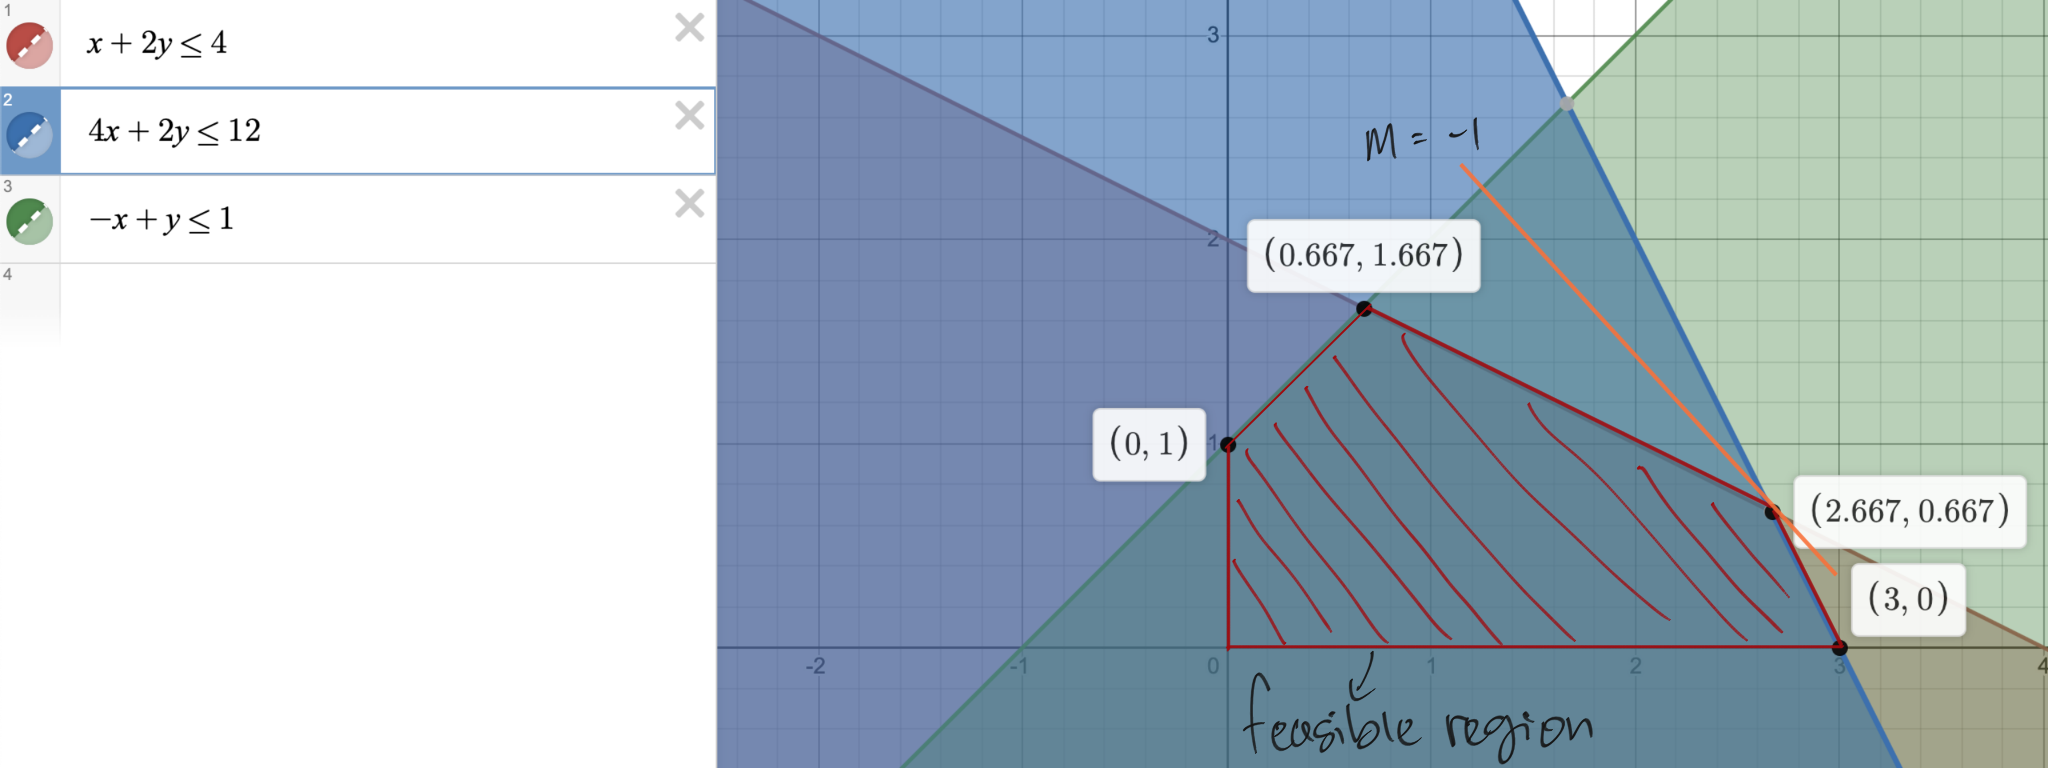
\includegraphics[scale=0.15]{./4a.png}
            \caption{Feasible region of $\vec{z}$.}
        \end{figure}
        {\color{blue}
            From the figure above, we can see that  $x = 2.667 \text{ and } y = 0.667$. 
            Thus, the optimal value is $z = x + y = 3.3333$.
        }

        \item (10\%) Derive its dual problem and solve the dual problem by any means. Compare the solutions of the primal and the dual problems.
        {\color{blue} 
            \begin{enumerate}
            \item The primal problem is as follow:

                Let $z$ be the optimal value, $x_i$ be the variables that we are planning to maximize, and $\omega_i$ be the slack variables.
                
                To solve the primal problem, we then convert it into a table. 
    
                The initial state
                \begin{center}
                    \begin{tabular}{ l } 
                        $ \zeta = x_1 + x_2 $ \\
                        \hline
                        $ \omega_1 = 4 - x_1 - 2x_2 $ \\
                        $ \omega_2 = 12 - 4x_1 - 2x_2 $ \\
                        $ \omega_3 = 1 + x_1 - x_2 $
                    \end{tabular}
                \end{center}
                
                The first iteration
                \begin{center}
                    \begin{tabular}{ l } 
                        $\zeta = 3 + \frac{1}{2}x_2 - \frac{1}{4}\omega_2$ \\
                        \hline
                        $\omega_1 = 1 - \frac{3}{2}x_2 + \frac{1}{4}\omega_2$ \\
                        $x_1 = 3 - \frac{1}{2}x_2 - \frac{1}{4}\omega_2$ \\
                        $\omega_3 = 4 - \frac{3}{2}x_2 - \frac{1}{4}\omega_2$ \\
                    \end{tabular}
                \end{center}
    
                The second iteration
                \begin{center}
                    \begin{tabular}{ l } 
                        $\zeta = \frac{10}{3} - \frac{1}{6}\omega_2 - \frac{1}{3}\omega_1$ \\
                        \hline
                        $x_2 = \frac{2}{3} + \frac{1}{6}\omega_2 - \frac{2}{3}\omega_1$ \\
                        $x_1 = \frac{8}{3} - \frac{1}{3}\omega_2 + \frac{1}{3}\omega_1$ \\
                        $\omega_3 = 3 - \frac{1}{2}\omega_2 + \omega_1$ \\
                    \end{tabular}
                \end{center}

                The values of the slack variables are
                \[
                    \omega_1 = 0, \omega_2 = 0, \omega_3 = 3 
                \]
    
                The values of the decision variables are 
                \[
                    x_1 = \frac{8}{3} \\ x_2 = \frac{2}{3}
                \]

                The objective value
                \[
                    z = x_1 + x_2 = \frac{10}{3}
                \]

            \item The dual problem is
                \begin{equation}
                    \begin{aligned}
                        \min_{y_1, y_2, y_3} \quad & z = 4y_1 + 12y_2 + y_3 \\
                        \textrm{s.t.}   \quad & y_1 + 4y_2 - y_3 \geq 1 \\
                                        \quad & 2y_1 + 2y_2 + y_3 \geq 1 \\
                                        \quad & y_1, y_2, y_3 \geq 0 \\
                    \end{aligned}
                \end{equation}

                Let $s_i$ be the surplus variables and $a_i$ be the artificial variables. Including these variables in the dual problem, we then have
                \begin{equation}
                    \begin{aligned}
                        \min \quad & z = 4y_1 + 12y_2 + y_3 + 0s_1 + 0s_2 + Ma_1 + Ma_2 \\
                        \textrm{s.t.}   \quad & y_1 + 4y_2 - y_3 - s_1 + a_1 =  1 \\
                                        \quad & 2y_1 + 2y_2 + y_3 - s_2 + a_2 = 1 \\
                                        \quad & y_1, y_2, y_3, s_1, s_2, a_1, a_2 \geq 0 \\
                    \end{aligned}
                \end{equation}

                Since we want to solve the dual problem above, we then convert the equations above into a table and 2 iterations are needed to find the optimal solution.

                \begin{figure}[H]
                    \centering
                    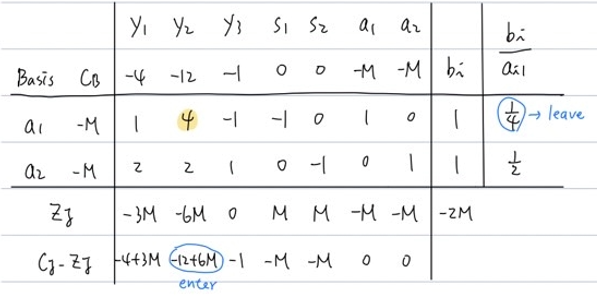
\includegraphics[scale=0.6]{./dual1.png}
                    \caption{The initial state.}
                \end{figure}

                \begin{figure}[H]
                    \centering
                    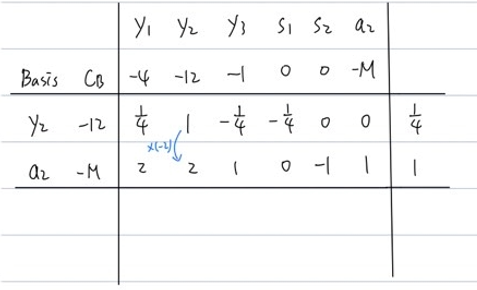
\includegraphics[scale=0.6]{./dual2.png}
                    \caption{The first iteration (1).}
                \end{figure}

                \begin{figure}[H]
                    \centering
                    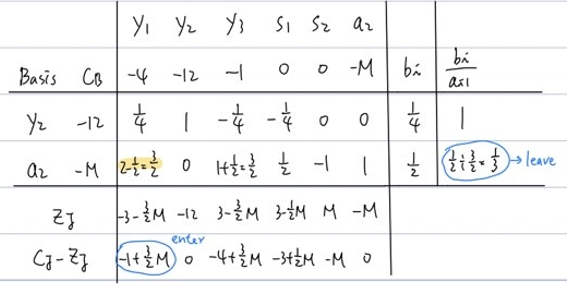
\includegraphics[scale=0.6]{./dual3.png}
                    \caption{The first iteration (2).}
                \end{figure}

                \begin{figure}[H]
                    \centering
                    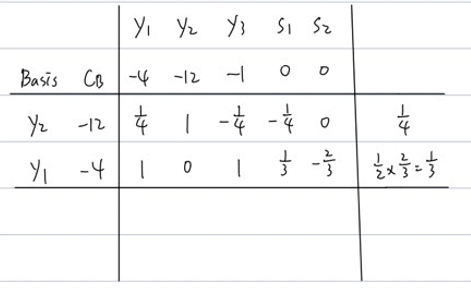
\includegraphics[scale=0.6]{./dual4.png}
                    \caption{The last iteration (1).}
                \end{figure}
                
                \begin{figure}[H]
                    \centering
                    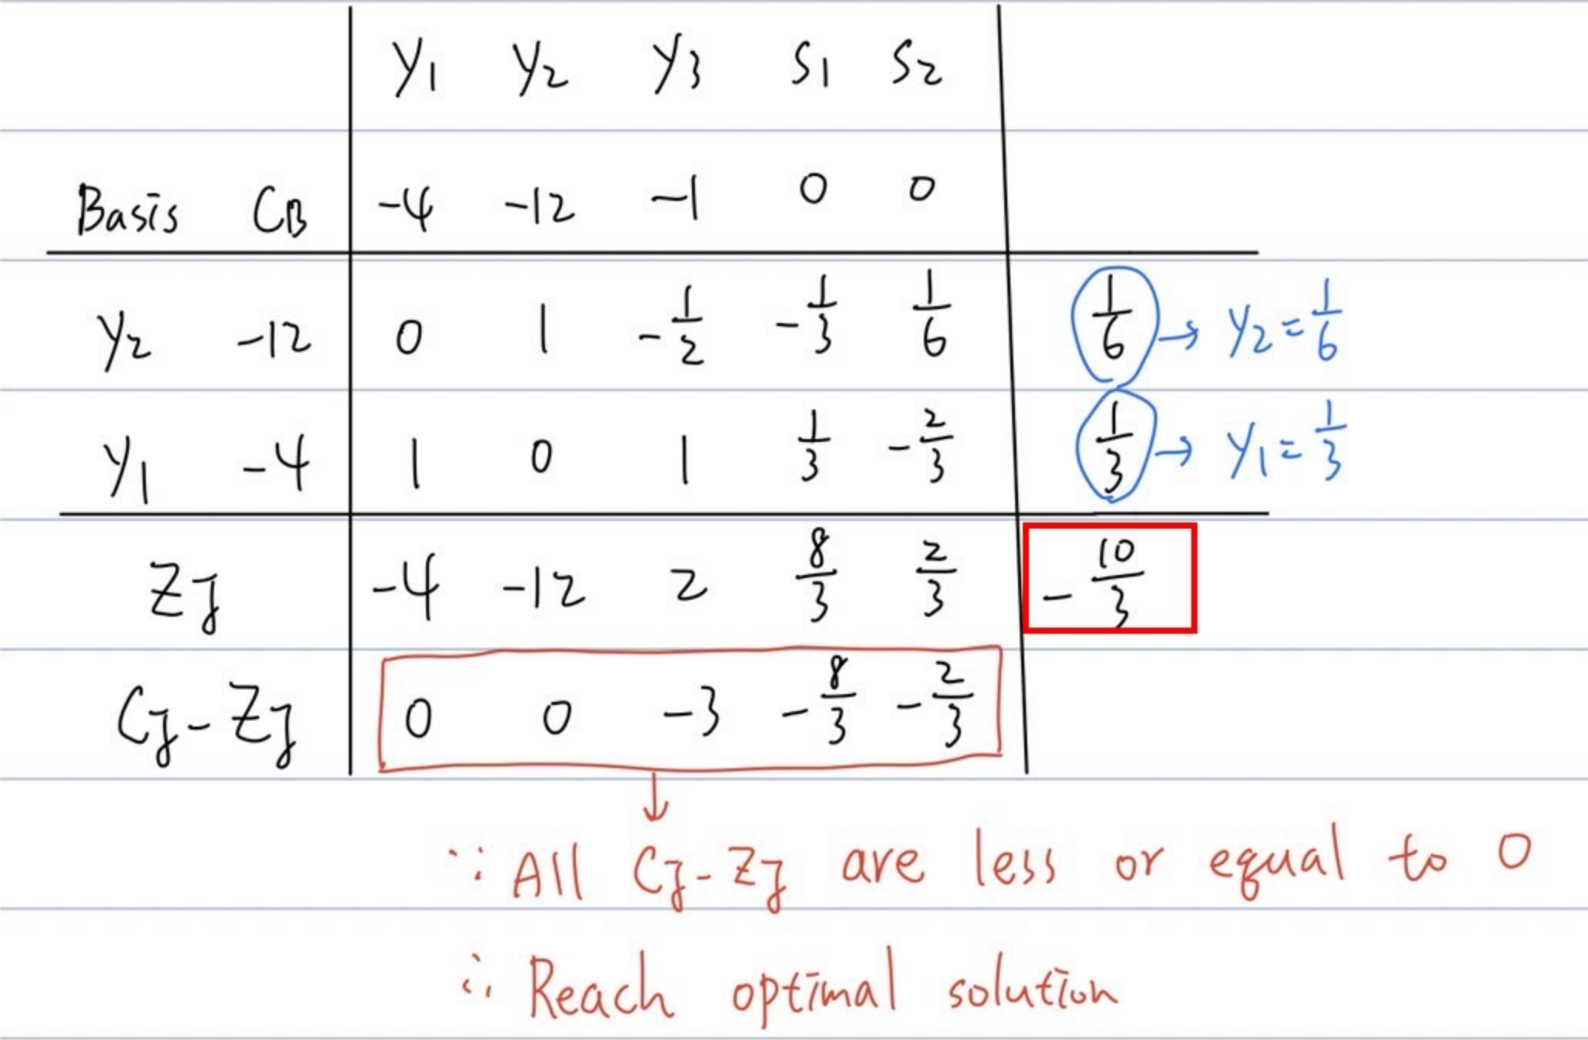
\includegraphics[scale=0.3]{./dual5.png}
                    \caption{The last iteration (2).}
                \end{figure}

                Thus, the objective value for the dual problem is $-(-\frac{10}{3}) = \frac{10}{3}$.
            \end{enumerate}

            From the solutions that we get from the primal problem and the dual problem,
            we can infer that the values of surplus variables in the dual problem equal to the values of decision variables in the primal problem.
            
            As for the optimal values of the primal slack variables are the first three entries in the $C_j - Z_j$ row. Thus,
            \begin{align}
                \omega_1 &= -(\text{first entry of }C_j - Z_j) = 0 \\
                \omega_2 &= -(\text{second entry of }C_j - Z_j) = 0 \\ 
                \omega_3 &= -(\text{third entry of }C_j - Z_j) = 3  
            \end{align}
            
            Most importantly, we can observe that the optimal value of the objective function is the same for both primal and dual.
        }

        \item (10\%) Verify the complementarity slackness condition.
        {\color{blue}
            Suppose that $x = (x_1, x_2, \ldots, x_n)$ is a {\color{red}primal feasible} solution and $y = (y_1, y_2, \ldots, y_n)$ is a {\color{red}dual feasible} solution. 
            Let $(\omega_1, \omega_2, \ldots, \omega_m)$ be the corresponding primal slack variables, and $(z_1, z_2, \ldots, z_n)$ be the corresponding dual slack variables.
            Then {\color{red} $x$ and $y$ are optimal} for their respective problems if and only if:
            \begin{enumerate}
                \item $z_j \cdot x_j = 0 \text{, for } j = 1, 2, \ldots, n$
                \item $\omega_i \cdot y_i = 0 \text{, for } i = 1, 2, \ldots, m$
            \end{enumerate} 

            For the primal problem, 
            \begin{align}
                z_1 \cdot x_1 = 0 \cdot \frac{8}{3} = 0 \\
                z_2 \cdot x_2 = 0 \cdot \frac{2}{3} = 0
            \end{align}

            For the dual problem, 
            \begin{align}
                \omega_1 \cdot y_1 = 0 \cdot \frac{1}{3} = 0 \\
                \omega_2 \cdot y_2 = 0 \cdot \frac{1}{6} = 0
            \end{align}
        }

        \item (10\%) Transform the problem to the standard form.
        {\color{blue} 
            \begin{equation}
                \begin{aligned}
                    \min_{x_1,x_2} \quad & z = - x_1 - x_2 \\
                    \textrm{s.t.} \quad & x_1 + 2x_2 + x_3 = 4 \\
                        \quad & 4x_1 + 2x_2 + x_4 =  12   \\
                        \quad & -x_1 + x_2 + x_5 = 1  \\
                        \quad & x_1, x_2, x_3, x_4, x_5 \geq 0
                \end{aligned}
            \end{equation}
        }

        \item (10\%) Solve it by the simplex method, as provided in Figure 1, using $\vec{x}_0 = (0, 0)$.
        Indicate $B_k, N_k, \vec{s}_k, \vec{d}_k, p_k, q_k, \gamma_k$ in each step.\
        
        {\color{blue} 
            Let $\mathcal{B} = \begin{bmatrix} 3 & 4 & 5 \end{bmatrix}$ be the index set of the basic variables and $\mathcal{N} = \begin{bmatrix} 1 & 2 \end{bmatrix}$ the index set of the non-basic variables.
            \begin{enumerate}
                \item Iteration 1
                    \[ B = \begin{bmatrix}1 & 0 & 0 \\ 0 & 1 & 0 \\ 0 & 0 & 1\end{bmatrix}, N =  \begin{bmatrix}1 & 2 \\ 4 & 2 \\ -1 & 1 \end{bmatrix}\]
                    \begin{align}
                        \vec{x}_N &= \begin{bmatrix} 0 \\ 0 \end{bmatrix} \\
                        \vec{X}_B &= B^{-1}b = b = \begin{bmatrix} 4 \\ 12 \\ 1 \end{bmatrix} \\
                        \vec{x} &= \begin{bmatrix} \vec{x}_B \\ \vec{x}_N \end{bmatrix}
                        = \begin{bmatrix} x_3 \\ x_4 \\ x_5 \\ x_1 \\ x_2 \end{bmatrix} 
                        = \begin{bmatrix} 4 \\ 12 \\ 1 \\ 0 \\ 0 \end{bmatrix} 
                    \end{align}

                    Solve $\vec{v}$ in $B^T\vec{v} = \vec{c}_B$. Thus, 
                    \[
                        \vec{v} = \begin{bmatrix} 0 \\ 0 \\ 0 \end{bmatrix}
                    \]

                    Pricing vector 
                    \[
                        \vec{p} = \vec{c}_N - N^T\vec{v} = \begin{bmatrix} -1 \\ -1 \end{bmatrix}
                    \]

                    Solve $B\vec{s}=A(:,1)$ to check if it is bounded
                    \begin{align}
                        \vec{s} &= B^{-1}\vec{A}_1 = \begin{bmatrix} 1 \\ 4 \\ -1 \end{bmatrix} > 0 \\
                        \vec{d} &= \begin{bmatrix} d_3 \\ d_4 \\ d_5 \\ d_1 \\ d_2 \end{bmatrix} = \begin{bmatrix} -1 \\ -4 \\ -1 \\ 1 \\ 0 \end{bmatrix}
                    \end{align}

                    Ratio test 
                    \[
                        \alpha = \min(|\frac{4}{-1}|, |\frac{12}{-4}|) = 3
                    \]

                    Thus, 
                    \begin{align}
                        \vec{x}_B^{new} &= \vec{x}_B^{old} - \alpha \vec{s} = \begin{bmatrix} 4 \\ 12 \\ 1 \end{bmatrix} - 3 \begin{bmatrix} 1 \\ 4 \\ -1 \end{bmatrix} =  \begin{bmatrix} 1 \\ 0 \\ 4 \end{bmatrix} \\
                        \vec{x}^{new} &= \begin{bmatrix} x_3 \\ x_1 \\ x_5 \\ x_4 \\ x_2 \end{bmatrix} \\
                        \vec{B}^{new} &= \begin{bmatrix}1 & 1 & 0 \\ 0 & 4 & 0 \\ 0 & -1 & 1\end{bmatrix} \\
                        N^{new} &= \begin{bmatrix} 0 & 2 \\ 1 & 2 \\ 0 & 1 \end{bmatrix} \\
                        A^{new} &= \begin{bmatrix} 0 & 2 & 1 & 1 & 0 \\ 1 & 2 & 0 & 4 & 0 \\ 0 & 1 & 0 & -1 & 1 \end{bmatrix}
                    \end{align}

                    The index set of the new basic variables are $\mathcal{B} = \{3,1,5\}$ and the non-basic variables are $\mathcal{N} = \{4,2\}$ 
                
                \item Iteration 2
                    \begin{align}
                        \vec{x}_N &= \begin{bmatrix} 0 \\ 0 \end{bmatrix} \\
                        \vec{X}_B &= B^{-1}b = b \\
                        &= \begin{bmatrix} 1 & -1/4 & 0 \\ 0 & 1/4 & 0 \\ 0 & 1/4 & 1 \end{bmatrix} \begin{bmatrix} 4 \\ 12 \\ 1 \end{bmatrix} = \begin{bmatrix} 1 \\ 3 \\ 4 \end{bmatrix}
                    \end{align}
                    
                    Solve $\vec{v}$ in $B^T\vec{v} = \vec{c}_B$. Thus, 
                    \begin{align}
                        B^T\vec{v} &= \vec{c}_B \\
                        &= \begin{bmatrix} 1 & -1/4 & 0 \\ 0 & 1/4 & 0 \\ 0 & 1/4 & 1 \end{bmatrix} \begin{bmatrix} v_1 \\ v_2 \\ v_3 \end{bmatrix} = \begin{bmatrix} 0 \\ -1 \\ 0  \end{bmatrix} \\ 
                        \vec{v} &= \begin{bmatrix} 0 \\ -1/4 \\ 0 \end{bmatrix}
                    \end{align}

                    Pricing vector 
                    \begin{align}
                        \vec{p} &= \vec{c}_N - N^T\vec{v} \\
                        &= \begin{bmatrix} 0 \\ -1 \end{bmatrix} - \begin{bmatrix} 0 & 1 & 0 \\ 2 & 2 & 1 \end{bmatrix} \begin{bmatrix} 0 \\ -1/4 \\ 0 \end{bmatrix} \\
                        &= \begin{bmatrix} 1/4 \\ -1/2 \end{bmatrix}
                    \end{align}

                    Solve $B\vec{s}=A(:,2)$ to check if it is bounded
                    \begin{align}
                        \vec{s} &= B^{-1}\vec{A}_2 \\
                        \begin{bmatrix} 1 & -1/4 & 0 \\ 0 & 1/4 & 0 \\ 0 & 1/4 & 1 \end{bmatrix} \begin{matrix} 2 \\ 2 \\ 1 \end{matrix} &= \begin{matrix} 3/2 \\ 1/2 \\ 3/2 \end{matrix} > 0 \\
                        \vec{d} &= \begin{bmatrix} d_3 \\ d_1 \\ d_5 \\ d_4 \\ d_2 \end{bmatrix} = \begin{bmatrix} -3/2 \\ -1/2 \\ -3/2 \\ 0 \\ 1 \end{bmatrix}
                    \end{align}

                    Ratio test 
                    \[
                        \alpha = \min(|-\frac{2}{3}|, |6|, |\frac{8}{3}|) = \frac{2}{3}
                    \]

                    Thus, 
                    \begin{align}
                        \vec{x}^{new} &= \begin{bmatrix} x_2 \\ x_1 \\ x_5 \\ x_3 \\ x_2 \end{bmatrix} \\
                        \vec{B}^{new} &= \begin{bmatrix} 2 & 1 & 0 \\ 2 & 4 & 0 \\ 1 & -1 & 1\end{bmatrix} \\
                        N^{new} &= \begin{bmatrix} 0 & 1 \\ 1 & 0 \\ 0 & 0 \end{bmatrix} \\
                        A^{new} &= \begin{bmatrix} 0 & 1 & 2 & 1 & 0 \\ 1 & 0 & 2 & 4 & 0 \\ 0 & 0 & 1 & -1 & 1 \end{bmatrix}
                    \end{align}

                    The index set of the new basic variables are $\mathcal{B} = \{2,1,5\}$ and the non-basic variables are $\mathcal{N} = \{4,3\}$ 
                
                \item Iteration 3
                    \begin{align}
                        \vec{x}_N &= \begin{bmatrix} 0 \\ 0 \end{bmatrix} \\
                        \vec{X}_B &= B^{-1}b = b \\
                        &= \begin{bmatrix} 2/3 & -1/6 & 0 \\ -1/3 & 1/3 & 0 \\ -1 & 1/2 & 1 \end{bmatrix} \begin{bmatrix} 4 \\ 12 \\ 1 \end{bmatrix} = \begin{bmatrix} 2/3 \\ 8/3 \\ 3 \end{bmatrix}
                    \end{align}

                    Solve $\vec{v}$ in $B^T\vec{v} = \vec{c}_B$. Thus, 
                    \begin{align}
                        B^T\vec{v} &= \vec{c}_B \\
                        \begin{bmatrix} 2 & 2 & 1 \\ 1 & 4 & -1 \\ 0 & 0 & 1 \end{bmatrix} \begin{bmatrix} v_1 \\ v_2 \\ v_3 \end{bmatrix} &= \begin{bmatrix} 0 \\ -1 \\ 0  \end{bmatrix} \\ 
                        \vec{v} &= \begin{bmatrix} -1/3 \\ -1/6 \\ 0 \end{bmatrix}
                    \end{align}

                    Pricing vector 
                    \begin{align}
                        \vec{p} &= \vec{c}_N - N^T\vec{v} \\
                        &= \begin{bmatrix} 0 \\ 0 \end{bmatrix} - \begin{bmatrix} 0 & 1 & 0 \\ 1 & 0 & 0 \end{bmatrix} \begin{bmatrix} -1/3\\ -1/6 \\ 0 \end{bmatrix} \\
                        &= \begin{bmatrix} 1/6 \\ 1/3 \end{bmatrix}
                    \end{align}

                    Since $\vec{p}$ is positive, the stopping condition is reached\dots

                    Thus, 
                    \begin{align}
                        \vec{x} &= \begin{bmatrix} \vec{x}_ 1 \\ \vec{x}_ 2 \end{bmatrix} = \begin{bmatrix} 8/3 \\ 2/3 \end{bmatrix} \\
                        z &= \frac{8}{3} + \frac{2}{3} = \frac{10}{3}
                    \end{align}

                    The maximum value is $10/3 = 3.333$.
            \end{enumerate}
        }
    \end{enumerate}

\begin{figure}[hb]
    \begin{center}
    \begin{tabular}{cp{.2in}l}
        \hline \\[0pt]
    (1) & \multicolumn{2}{l}{Given a basic feasible point $\vec{x}_0$ and the corresponding index set}\\
    & \multicolumn{2}{l}{ $\mathcal{B}_0$ and $\mathcal{N}_0$.} \\
    (2) & \multicolumn{2}{l}{For $k=0,1,\ldots$} \\
    (3) & & Let $B_k=A(:,\mathcal{B}_k), N_k=A(:,\mathcal{N}_k)$, $\vec{x}_B=\vec{x}_k(\mathcal{B}_k),
    \vec{x}_N=\vec{x}_k(\mathcal{N}_k)$, \\
        &  & and $\vec{c}_B=\vec{c}_k(\mathcal{B}_k), \vec{c}_N=\vec{c}_k(\mathcal{N}_k)$.\\
    (4) & & Compute $\vec{s}_k=\vec{c}_N-N_k^T{B_k^{-1}}^T\vec{c}_B$  \mbox{\color{blue} (pricing) } \\
    (5) & & If $\vec{s}_k\ge 0$, return the solution $\vec{x}_k$. \mbox{\color{blue} (found optimal solution) } \\
    (6) & & Select $q_k\in\mathcal{N}_k$ such that $\vec{s}_k(i_q)<0$, \\
        & & where $i_q$ is the index of $q_k$ in $\mathcal{N}_k$\\
    (7) & & Compute $\vec{d}_k={B^{-1}_k}A_k(:,q_k)$. \mbox{\color{blue} (search direction) } \\
    (8) & & If $\vec{d}_k\le 0$, return \verb"unbounded". \mbox{\color{blue} (unbounded case) } \\
    (9) & & Compute $\displaystyle [\gamma_k, i_p] = \min_{i,\vec{d}_k(i)>0}\frac{\vec{x}_B(i)}{\vec{d}_k(i)}$ \mbox{\color{blue} (ratio test) }\\
    &&\mbox{\color{blue} (The first return value is the minimum ratio;) }\\
    &&\mbox{\color{blue} (the second return value is the index of the minimum ratio.) } \\
    (10) & & $\displaystyle x_{k+1}\left(
                        \begin{array}{c}
                        \mathcal{B} \\
                        \mathcal{N} \\
                        \end{array}
                    \right) =  \left (\begin{array}{c}
                        \vec{x}_B \\
                        \vec{x}_N \\
                        \end{array}
                    \right) + \gamma_k \left (\begin{array}{c}
                        -\vec{d}_k \\
                        \vec{e}_{i_q} \\
                        \end{array}
                    \right)$ \\
    &&\mbox{\color{blue} ($\vec{e}_{i_q}={(0,\ldots,1,\ldots,0)}^T$ is a unit vector with $i_q$th element 1.)}\\
    (11) &&Let the $i_p$th element in $\mathcal{B}$ be $p_k$. \mbox{\color{blue} (pivoting) } \\
        & & $\mathcal{B}_{k+1} = (\mathcal{B}_k-\{p_k\})\cup\{q_k\}$,  $\mathcal{N}_{k+1}= (\mathcal{N}_k-\{q_k\})\cup\{p_k\}$  \\[10pt]
    \hline
    \end{tabular}
    \end{center}
    \caption{The simplex method for solving (minimization) linear programming}\label{}
\end{figure}

\end{enumerate}

\end{document}